\documentclass[10pt,a4paper]{beamer}
\usepackage[utf8]{inputenc}
%\usepackage[spanish]{babel}
\usepackage{amsmath}
\usepackage{amsfonts}
\usepackage{amssymb}
\usepackage{makeidx}
\usepackage{graphicx}
\usepackage{makecell}
\usepackage{verbatim}
\author{Cristian Chimbo}
\usefonttheme{professionalfonts} % fuentes de LaTeX
\usetheme{Szeged}
\usecolortheme{beaver}
\setbeamercovered{transparent}
\begin{document}
%\font\myfont=cmr12 at 20pt
%\title{{\myfont Precise Weed and Maize Classification through Convolutional Neuronal Networks}}
%\author{{\bf C\'ordova Andrea\inst{1}, Barreno Mauricio, J\'acome Jos\'e }\\
%\institute{
%\inst{1}%
 % Universidad de las Fuerzas Armadas ESPE\\
 % Latacunga - Ecuador}
%{ 2nd IEEE Ecuador Technical Chapters Meeting}
%\vspace*{1cm}}
%\date{October 2017}
\title[Precise Weed and Maize Classification through Convolutional Neuronal Networks] %optional
{Precise Weed and Maize Classification through
Convolutional Neuronal Networks}
 
 
\author[C\'ordova Andrea, Barreno Mauricio and J\'acome Jos\'e] % (optional, for multiple authors)
{C\'ordova Andrea, Barreno Mauricio and J\'acome Jos\'e}
 
\institute[Universidad de las Fuerzas Armadas ESPE] % (optional)
{
  \inst{1}%
  Departamento de Energ\'ia y Mec\'anica\\
  Universidad de las Fuerzas Armadas ESPE
}
 
\date[Ecuador] % (optional)
{2nd IEEE Ecuador Technical Chapters Meeting, October 2017}
\frame{\titlepage}
%-----------------------------
\begin{frame}
\frametitle{Presentation Outline}
\tableofcontents
%\newpage
\end{frame}
%-----------------------------
\section{Introduction}
\begin{frame}
\frametitle{Introduction}
\begin{enumerate}
\item Maize is one of the most important food of the world.
\item Las malas hierbas en el maiz pueden afectan hasta 5000 Kg/Hectaria de produccion.
\item La robotica esta presentando grandes avances en la agricultura de precision.
\item Inteligencia artificial cada vez se acerca mas a la inteligencia humana.\\
\end{enumerate}
\end{frame}
%--------------
\section{The Propose of the present study}
\begin{frame}
\frametitle{The Propose of the present study}
\begin{enumerate}
\item Obtener muestras(imagenes) para conformar un dataset.
\item Segmentar las muestras.
\item Probar diferentes arquitecturas de Redes Neuronales Convolucionales para entrenar la red.
\item Hacer Benchmark en diferentes hardwares para analizar tiempos de procesamiento.
\item Optimizar la red.
\end{enumerate}
\end{frame}
%-----------------------------
\section{Hardware and Software Used}
\begin{frame}
\frametitle{Hardware and Software Used}
\textbf{Hardware}
\begin{enumerate}
\item Raspberry Pi 3.
\item Pi camera V2.1.
\item Nvidia graphic Card GTX950M.
\end{enumerate}
\textbf{Software}
\begin{enumerate}
\item OpenCV Library
\item Caffe framework
\item Ubuntu 16.04
\item PIXEL Distribution derived from Debian.
\end{enumerate}
\end{frame}
%-----------------------------
\section{Image Processing}
\begin{frame}
\begin{itemize}
	\item Acquire  an RGB image through RPi Camera v2.1
	\item Detect contours and crop image to the contour
	\item Normalize Green Channel and then $S = 2*G - R - B$ \footnote{Poner cita aqui}
	\item OTSU Thresholding
	\item Mask image
\end{itemize}
\frametitle{Image Processing}
	\begin{figure}[h]
	\centering
	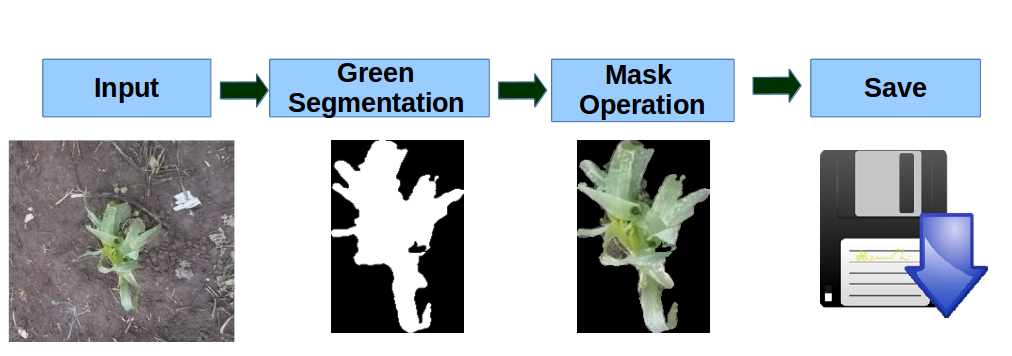
\includegraphics[width=3.5 in]{procesamiento}
	\caption{The process of image processing, por lo pronto}
	\label{figure4}
	\end{figure}
\end{frame}
%-----------------------------
\section{Dataset}
\begin{frame}
\frametitle{Dataset}
{Dataset Description}
\begin{enumerate}
\item Place Pillaro Tungurahua Ecuador
\item La imagenes fueron obtenidas encampos de maiz en su estapa inicial,( plantas con 3 a 7 hojas) \cite{sladojevic2016deep}.
\item Imagenes rotadas cada 30 para mejorar la deteccion de las planta.
\item 1/5 del total de las imagenes al azar fueron usadas para la etapa de validacion
\end{enumerate}
\begin{table}[h!]
\renewcommand{\arraystretch}{1.3}
\caption{Dataset distribution of each class}
\label{table:1}
\centering
\begin{tabular}{| c c c |} 
 \hline
 \textbf{Images} & \textbf{Maize} & \textbf{Weed}  \\ [1ex] 
 \hline
 Original  & 2835 & 880 \\ 
 Rotated & 34222 & 10762 \\ 
 Entrenamiento & 25695 & 8560 \\
 Validacion & 8325 & 2000 \\
 \hline
\end{tabular}
\end{table}
\end{frame}
%-----------------------------
\section{Convolutional Neural Networks}
\begin{frame}
\frametitle{Convolutional Neural Networks(CNN)}
\begin{itemize}
	\item Highly accurate method for image classification
	\item A class of deep, feed-forward artificial neural networks
	\item Tested on classification of plants, poner citas
	\item Multiple architectures and applications
\end{itemize}
	\begin{figure}[h]
	\centering
	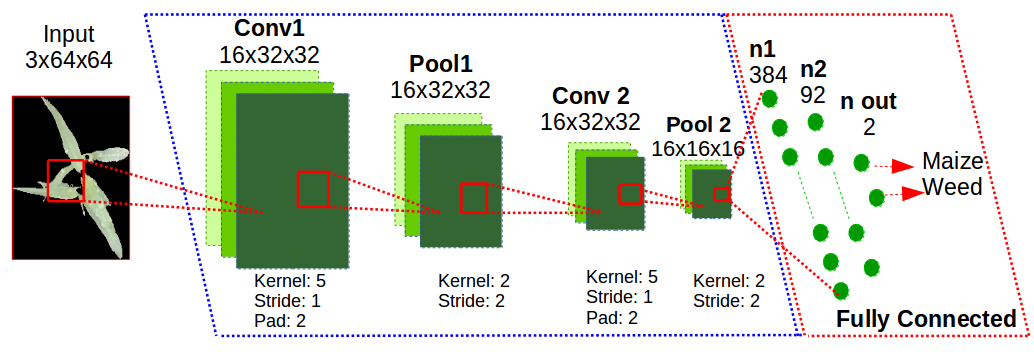
\includegraphics[width=3.5 in]{arquitectura}
	\caption{Normal architecture in a Convolutional Neural Network}
	\label{figure4}
	\end{figure}
\end{frame}
\section{Architectures Tested}
\begin{frame}
\frametitle{Architectures tested}
\begin{itemize}
	\item Highly accurate method for image classification
\end{itemize}
\begin{table}[h!]
\centering
\renewcommand{\arraystretch}{1.2}
\caption{Comparison of the 4 types of CNN}
\label{table:2}
\begin{tabular}{|l c c c c|} 
 \hline
 \textbf{Parameters }& \textbf{LeNet} & \textbf{AlexNet} & \textbf{cNET} & \textbf{sNET} \\ [0.75ex] 
 \hline
 Input size of images & 32x32 & 64x64 & 64x64 & 64x64 \\ 
 Layers numbers & 9 & 11 & 8 & 4\\
 Number of parameters & 652500 & 20166688 & 6421568 & 135872 \\ 
 Iterations & 3000 & 3000 & 3000 & 3000 \\ 
 Accuracy(\%) & 86.48 & 93.86 & 96.4 & 80.4 \\
 Loss(\%) & 32.80 & 15.32 & 13.72 & 15.32 \\ [1ex] 
 \hline 
\end{tabular}
\end{table}
\end{frame}
%-----------------------------
\section{cNET Performance}
\begin{frame}
\frametitle{cNET Performance}
\begin{enumerate}
\item Obtener muestras(imagenes) para conformar un dataset.
\end{enumerate}
\begin{table}[h!]
\centering
\renewcommand{\arraystretch}{1.2}
\caption{Test of cNET 16 filters with optimized software}
\label{table:5}
\begin{tabular}[c c c c]{|p{2.2 cm} p{1.1cm} p{1.1cm} p{2.4cm}|} 
 \hline
 \textbf{Hardware } & \textbf{Accuracy Weed} & \textbf{Accuracy Maize} & \textbf{Average time of classification/image}\\ 
 \hline 
 GPU & 92.08\% & 89.11\% & 1.58 ms \\ [0.95ex]
 CPU & 92.08\% & 89.11\% & 10.92 ms \\ [0.95ex]
 CPU(Raspberry Pi) & 92.08\% & 89.11\% & 150.8 ms \\ [0.95ex]
 \hline
\end{tabular}
\end{table}
\end{frame}
%-----------------------------
\section{Presuming performance of cNET 16 filters}
\begin{frame}
\frametitle{Presuming performance of cNET 16 filters}
\begin{table}[h!]
\centering
\renewcommand{\arraystretch}{1.2}
\caption{Test of complete image classification in FPS}
\label{table:6}
\begin{tabular}[c c c c]{|p{1.0 cm} p{1.7cm} p{1.7cm} p{1.7cm}|} 
 \hline
 \textbf{Parameter} &\textbf{GPU } & \textbf{CPU} & \textbf{Raspberry Pi} \\ 
 \hline
 Time(s) & 0.0171 & 0.196 & 2.714 \\ [0.95ex]
 FPS & 58.47 & 5.08 & 0.36 \\ [0.95ex]
 \hline
\end{tabular}
\end{table}
\end{frame}
%--------------
\section{Conclusion}
\begin{frame}
\frametitle{Conclusion}
\begin{itemize}
\item
\item
\end{itemize}
\end{frame}
%--------------
\section{Recomendations}
\begin{frame}
\frametitle{Recomendations}
\begin{itemize}
\item
\item
\end{itemize}
\end{frame}
%--------------
\large
\begin{frame}
%\frametitle{The Propose of the present study}
\begin{center}
Thanks!
\end{center}
\end{frame}

%-----------------------------
\bibliographystyle{plain}
\bibliography{bibliografiapaper}
\end{document}
